\documentclass{homework}
\usepackage[dvipsnames]{xcolor}
\usepackage{tikz}

\title{Assignment1: Probability}
\author{
  Dmitrii, Maksimov\\
  \texttt{dmitrii.maksimov@fau.de} \\
  \texttt{ko65beyp}
  \and
  Ilia, Dudnik\\
  \texttt{ilia.dudnik@fau.de}\\
  \texttt{ex69ahum}
  \and
  Aleksandr, Korneev\\
  \texttt{aleksandr.korneev@fau.de}\\
  \texttt{uw44ylyz}
}
\begin{document}

\maketitle

\exercise[1.2 (Disjunctive Random Variables)]
\begin{align*}
	P(A\lor B \lor C) &= P(A\lor B) + P(C) - P((A\lor B)\land C)  \\
	&= P(A) + P(B) - P(A\land B) + P(C) - P(A\land C \lor B \land C) \\
	&= P(A) + P(B) + P(C) - P(A\land B) - P(A\land C) - P(B \land C) + P(A\land B \land C)
\end{align*}
Corresponding Venn diagram:
 \begin{figure}[!h]
\centering
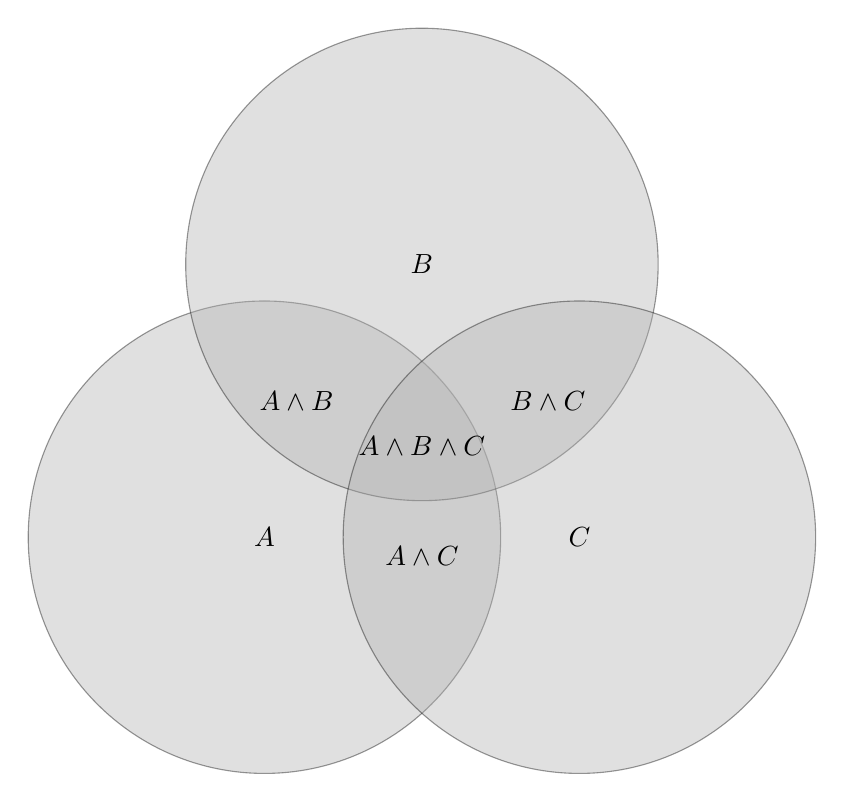
\begin{tikzpicture} [set/.style = {draw,
    circle,
    minimum size = 6cm,
    fill=black!30,
    opacity = 0.4,
    text opacity = 1}]
 
\node (A) [set] {$A$};
\node (B) at (60:4cm) [set] {$B$};
\node (C) at (0:4cm) [set] {$C$};
 
\node at (barycentric cs:A=1,B=1) [left] {$A\land B$};
\node at (barycentric cs:A=1,C=1) [below] {$A\land C$};
\node at (barycentric cs:B=1,C=1) [right] {$B \land C$};
\node at (barycentric cs:A=1,B=1,C=1) [] {$A\land B \land C$};
 
\end{tikzpicture}
\end{figure}

\end{document}